\documentclass{article}
\usepackage{tikz}
\usetikzlibrary{arrows.meta,arrows}
\begin{document}
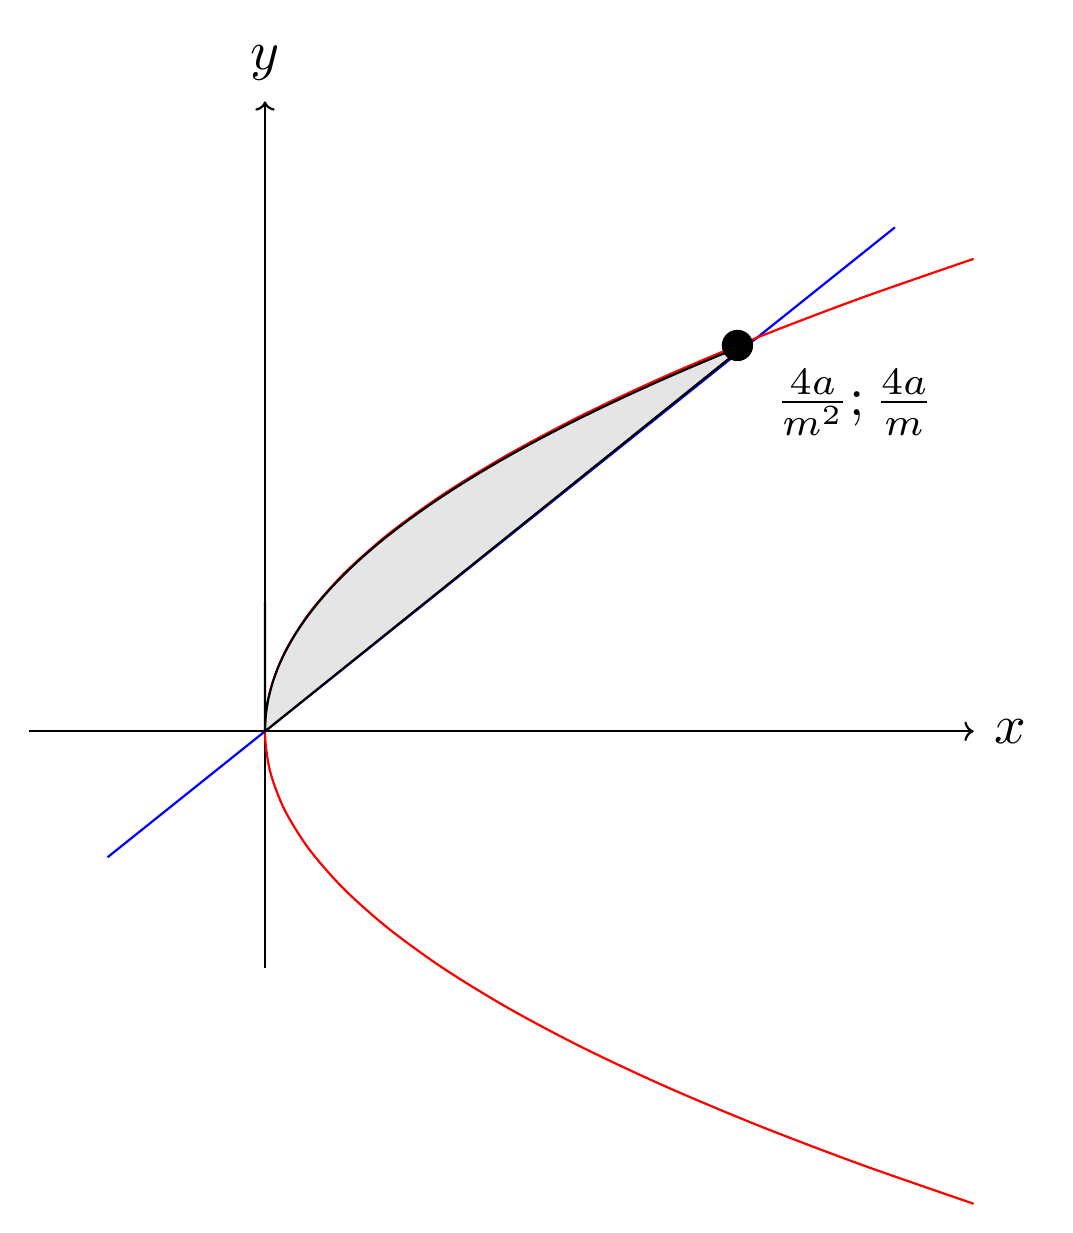
\begin{tikzpicture}[thick,scale=1, every node/.style={scale=2}]


\draw[->] (-3, 0) -- (9, 0) node[right] {$x$};
\draw[->] (0, -3) -- (0, 8) node[above] {$y$};

% draw the curves
\draw[ domain=-2:8, smooth, variable=\x, blue] plot ({\x}, {0.8*\x});
\draw[ domain=-3:3, smooth, variable=\y, red]  plot ({\y*\y}, {2*\y});

% draw the area between the curves
\draw[fill=gray!20,scale=0.82, domain=0:3, smooth, variable=\y] plot ({0.83*\y*\y}, {2*\y}) -- (0,0) -- (0,2) -- cycle;

\node[circle, fill=black,inner sep=2pt,label=-10:\color{black}$\frac{4a}{m^2};\frac{4a}{m}$]at (6,4.9){};

\end{tikzpicture}
\end{document}
